\chapter{A single step evolution model driven by digital Elastica minimization}
\chaptermark{A single step evolution model}
\label{chapter:balance-flow}


In this chapter we introduce the balance coefficient, a value that indicates how far the intersection of some ball and a digital shape is from half of the ball area. This value motivates the definition of a new family of energies to regularize the squared curvature: the $m$-BalanceFlow. We are going to show that the BalanceFlow is closely related to the FlipFlow energy, but the former has an easier interpretation and leads to a simpler algorithm to implement.


\section{BalanceFlow model}
In~\cref{ch6:subsec:flipflow-algorithm-discussion}, we have argued that inverting the solution was necessary to reduce the squared curvature estimation in the next shape of the flow. In this section, we investigate further the reasons involved in this unusual inversion step. 

\subsection{Definitions}

In the FlipFlow model no contour information is given, and the strategy there were to label the pixels such that the next shape has a boundary in which the estimation balls were more balanced than in the previous shape, i.e., the difference $|B_r(p) \cap \Ds| - |B_r(p) \cap \overline{\Ds}|$ is closer to zero for every pixel $p \in \partial \Ds$.  We formalize this idea by defining the balance coefficient.

\begin{definition}{Balance coefficent}
Given digital shape $\Ds \in \Omega$, positive number $r$ and point $p \in \Omega$, the \emph{balance coefficient} of $\Ds$ at $p$ is defined as
\begin{align*}
	u_r(\Ds,p) = \left( \frac{\pi r^2}{2} - |B_r(p) \cap \Ds| \right)^2.
\end{align*}
%
\end{definition}

The balance coefficient definition is very similar to the II squared curvature estimator. Nonetheless, we have decided to make a new definition since we do not have the scaling factor $\frac{9}{R^6}$ and that the balance coefficient can be computed everywhere and not only in the digital boundary of the shape. Let $F=B_r(p) \cap \Ds$ and $G=B_r(p) \setminus F$. The balance coefficient is symmetric with respect $F$ and $G$. 
\begin{align*}
	u_r(\Ds,p) &= \left( \frac{\pi r^2}{2} - |F| \right)^2 = \left( -\frac{\pi r^2}{2} + |G| \right)^2 = \left( \frac{\pi r^2}{2} - |G| \right)^2.
\end{align*}
%
The balance coefficient is used to estimate the effect of moving the estimation ball center towards the interior or the exterior of the shape. For example, consider~\cref{fig:balance-plot} in which we plot the balance coefficients of points along the diagonal of a square shape. 

\begin{figure}
\center
\begin{minipage}{0.25\textwidth}
\subfloat{
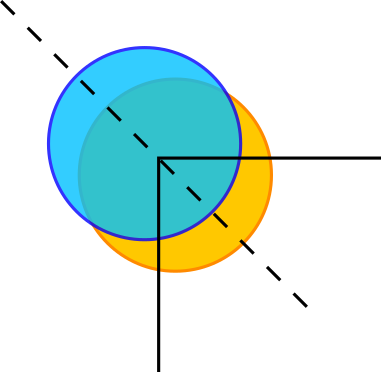
\includegraphics[scale=1.0]{figures/chapter7/distant-disks-1.png}}\\%
\subfloat{
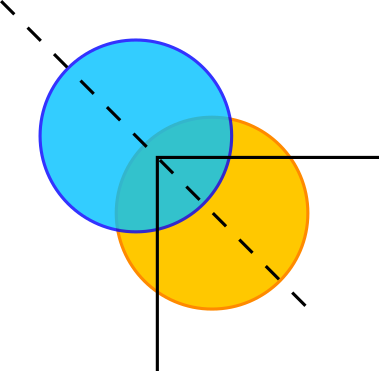
\includegraphics[scale=1.0]{figures/chapter7/distant-disks-2.png}}\\%
\subfloat{
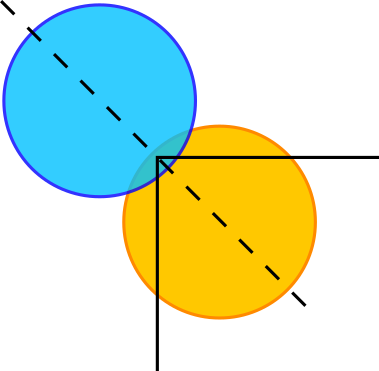
\includegraphics[scale=1.0]{figures/chapter7/distant-disks-3.png}}
\end{minipage}%
\begin{minipage}{0.75\textwidth}
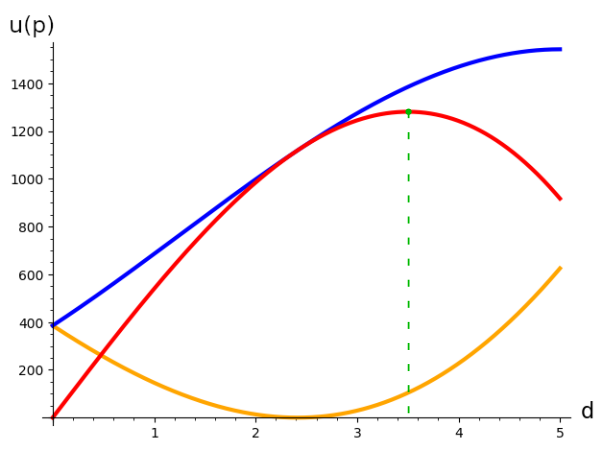
\includegraphics[scale=0.75]{figures/chapter7/balance-coefficient-p2-with-sum-2.png}
\end{minipage}
\caption{The balance coefficient $(r=5)$ of equidistant points from the corner of a square shape contour. The red curve indicates the difference between the blue and the orange curve. The inflexion point in the red curve indicates the point $p$ in which a ball centered at $p$ has balance coefficient equal to zero. The green point marks the point $p$ in which the difference between the balance coefficients is the greatest. }
\label{fig:balance-plot}
\end{figure}


The balance coefficient grows if the estimation ball is moved towards the exterior and decreases if the estimation ball is moved towards the interior of the shape. That is an indication that we should remove point $p$ from $\Ds$ to decrease the squared curvature of the shape at point $p \in \partial \Ds$. The same point $p$ may be touched by several balls, each of them contributing with some value for the ultimate decision of keep or remove point $p$ of $\Ds$. 
%The $m$-balance is defined as the sum of these contributions


%\begin{definition}{m-balance}
%Given digital shape $\Ds$, integer numbers $r>0, m \neq 0$, the \emph{m-balance} at point $p$ is defined as
%
%\begin{align*}
%	U_{m}(\Ds,p) &= \sum_{q \in Q_m(p)}{ u(\Ds,q)}
%\end{align*}
%
%where its zone of influence $Q_m(p)$ is defined as
%
%\begin{align*}
%	Q_m(p) &= \left\{\; q \in L_m(\Ds) \; | \; p \in B_r(q) \; \right\} \\
%\end{align*}
%
%\end{definition}
%
%\begin{figure}[h!]
%\center
%\includegraphics[scale=0.5]{figures/chapter7/k-balance.png}
%\caption{The $q$ points of the $m$-ring forms the zone of influence of the boundary point $p$.}
%\label{fig:balance-set}
%\end{figure}
%
%The zone of influence of $p$ is the set of all points $q$ in which $p$ is contained in the estimation ball centered at $q$. In the next section we define a flow that will have the following behaviour
%
%\begin{align*}
%	U_m(\Ds^{(k)},x_j) - U_{-m}(\Ds^{(k)},x_j) > 0 &\rightarrow x_j \notin \Ds^{(k+1)} \\
%	U_m(\Ds^{(k)},x_j) - U_{-m}(\Ds^{(k)},x_j) < 0 &\rightarrow x_j \in \Ds^{(k+1)}
%\end{align*}



We are going to consider the inner and outer pixel boundary simultaneously as the optimization variables. We recall that $\Ds^{(k)}$ corresponds to the digital shape $\Ds$ after the $k$-th iteration of the flow and that $d_{\Ds^{(k)}}$ is its signed distance transform. We list the sets needed to define the new family of energies:
\begin{align*}
	O^{(k)} &:=\left\{ p \in \Omega \; | \; -1 \leq d_{\Ds^{(k)}}(p) \leq 1 \right\}\\
	X^{(k)} &:= X(O^{(k)})  \\
	F^{(k)} &:= \Ds^{(k)} \setminus O^{(k)} \\
	F_r^{(k)}(p) &:= F^{(k)} \cap B_r(p)\\
	O_r^{(k)}(p) &:= O^{(k)} \cap B_r(p) \\
	X_r^{(k)}(p) &:= X\big( O_r^{(k)}(p) \big).
\end{align*}
%
We recall that an assignment of variables $X(\Omega)$ is denoted $x(\Omega)$. In case the shape is described in terms of a set of variables $X(\Omega)$, i.e., $\Ds=F \cup x(\Omega)$,  the balance coefficient is written as
\begin{align*}
	u_r(F,X,p) &=  \Big( \frac{\pi r^2}{2} - |F_r(p)| - \sum_{x_j \in X_r(p)}{x_j} \Big)^2.
\end{align*}
%
\subsection{Algorithm}

Let $p_i, p_o \in \mathcal{R}_m(\Ds)$ the inner and outer ball centers in the $m$-ring of $\Ds$, respectively. We assume $k=0$ if omitted, i.e., $\Ds=\Ds^{(0)}$. We define the term $T_{m}^{bal}(\Ds)$ as
\begin{align}
	T_{m}^{bal}(\Ds,X) &= \sum_{p_i,p_o \in \mathcal{R}_m(\Ds)}{u_r(F,1-X,p_o) - u_r(F,X,p_i)} \nonumber \\
	&=  \sum_{p_i,p_o \in \mathcal{R}_m(\Ds)}{\Bigg( \frac{\pi R^2}{2} - \Big(\; |F_o| + \sum_{ x_j \in X_o}{1-x_j} \; \Big) \Bigg)^2 -\Bigg(\frac{\pi R^2}{2} - \Big(\; |F_i| + \sum_{x_j \in X_i}{x_j}\;\Big)\Bigg)^2},
	\label{eq:balance-term}
\end{align}
%
where $X_o=X_r(p_o), X_i=X_r(p_i), F_o=F_r(p_o), F_i=F_r(p_i)$.


\cref{eq:balance-term} favors configurations of zero difference between the outer and inner ball coeficients, i.e., regions of zero curvature. In regions of positive curvature, the outer (inner) ball has a shortage (excess) of pixels, and minimization of~\cref{eq:balance-term} tends to label variables in these regions to zero (one).

The $m$-balance energy family is defined as
\begin{align}
  E_{(\vec{\theta},m)}^{bal}(\Ds^{(k)},X^{(k)}) =& \sum_{x_j \in X^{(k)}}{\alpha s(x_j)} + \beta T_{m}^{bal}(\Ds^{(k)},X^{(k)}) + \sum_{x_j \in X^{(k)}}{\gamma g(\Ds^{(k)},x_j)}.
  \label{eq:single-step-energy-family}
\end{align}
%
We follow the same notation of~\cref{chapter:flip-flow} to denote the data term $g(\Ds,x)$ and the length penalization term $s(x)$ that are defined as in~\cref{eq:length-penalization,eq:data-fidelity}, respectively. The BalanceFlow algorithm is summarized in~\cref{alg:balance-flow} and an illustration is shown in~\cref{fig:ch7-segmentation}.

\begin{algorithm}
 \SetKwData{It}{k}
 \SetKwData{MIt}{maxIt}
 \SetKwData{Delta}{delta}
 \SetKwInOut{Input}{input}\SetKwInOut{Output}{output}
 \SetKwComment{comment}{//}{}
 
 \Input{A digital set $\Ds$; The ring number $m$; parameter vector $\vec{\theta}=\alpha,\beta)$; data term coefficient $\gamma$; the maximum number of iterations \MIt;}
 \BlankLine
 $\Ds^{(0)} \longleftarrow \Ds$\;
 $k \longleftarrow 1$\;
 \While{ \It $<$ \MIt  }{ 	
	 	$x^{(k-1)} \longleftarrow \argmin_{X^{(k-1)}} E_{(\vec{\theta},m)}^{bal}(\Ds^{(k-1)},X^{(k-1)}) + \gamma g(X^{(k-1)})$\; 	
 		$\Ds^{(k)} \longleftarrow F^{(k-1)} + x^{(k-1)}$\;
 	
	\It $\longleftarrow$ \It $+1$\;
	
 }
 \caption{BalanceFlow algorithm.}
 \label{alg:balance-flow}  
\end{algorithm}

\begin{figure}
\center
\begin{tabular}{cccc}
\multirow{2}{*}{Seeds} & \multirow{2}{*}{GrabCut} & $\alpha=0.5, \beta=0.0,$ & $\alpha=0.5, \beta=1.0,$\\
& & $\gamma=2.0$ & $\gamma=2.0$\\
 	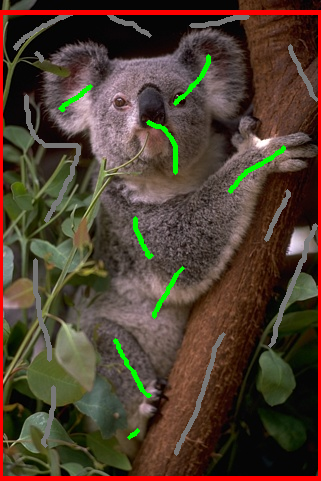
\includegraphics[scale=0.25]{figures/chapter7/segmentation/coala/k-0.0/seeds.png} & 
 	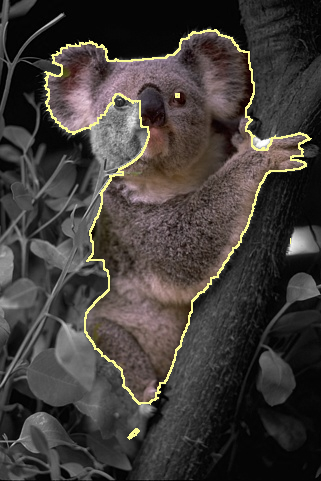
\includegraphics[scale=0.25]{figures/chapter7/segmentation/coala/k-0.0/gc-seg.png} &  	
 	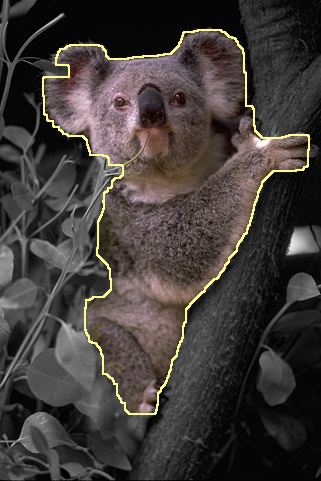
\includegraphics[scale=0.25]{figures/chapter7/segmentation/coala/k-0.0/corrected-seg.png} &  	
 	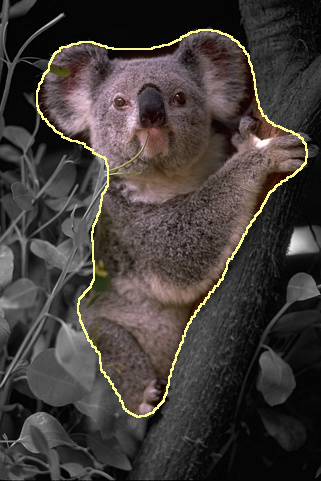
\includegraphics[scale=0.25]{figures/chapter7/segmentation/coala/k-1.0/corrected-seg.png}
\end{tabular}	
\caption{Given foreground (green) and background (gray) seeds at picture (a); GrabCut produces picture (b) which is used as input of the BalanceFlow algorithm; in pictures (c) and (d) we display the output of BalanceFlow algorithm with and without squared curvature regularization. }
\label{fig:ch7-segmentation}
\end{figure}


\section{Relation with FlipFlow}
	The BalanceFlow returns similar solutions to the FlipFlow algorithm, as the experiments in~\cref{chapter:results-analysis} illustrates. Indeed, they are closely related. We recall the curvature regularization term of the FlipFlow~\cref{eq:energy-family} for some digital shape $\Ds$ before proving proposition
\begin{align}
T_{m}^{flip}(D,X) &= \sum_{ p_i,p_o \in R_m(\Ds)}{ \Big( \frac{\pi R^2}{2} - F_r(p_o) - \sum_{x_j \in X_r(p_o)}{x_j}\Big)^2 + \Big(\frac{\pi R^2}{2} - F_r(p_i) - \sum_{x_j \in X_r(p_i)}{x_j}\Big)^2 }
\label{eq:curvature-term}
\end{align}
%
\begin{proposition}{FlipFlow and BalanceFlow relation}
The curvature terms of FlipFlow and BalanceFlow are related by the equality
\begin{align*}
T_{m}^{flip}(\Ds,1-X) &= T_{m}^{bal}(\Ds) + P_1(X_i) + c,
\end{align*}
where $P_1(X_i) = (\sum_{X_i}{ 1-x_j})^2 + (\sum_{X_i}{x_j})^2$ and $c$ is a constant.
\label{prop:flipflow-balanceflow-relation}
\end{proposition}

\begin{proof}

We replace $x_j$ by $(1-x_j)$ in~\cref{eq:curvature-term}, which corresponds to the complement of the solution in the FlipFlow model. To simplify notation, we are going to omit the radius $r$ and replace points $p_i,p_o$ by underscored $i,o$, i.e., $F_i := F_r(p_i)$. We rewrite~\cref{eq:curvature-term} as
\begin{align}
T_{m}^{flip}(\Ds,1-X) &= \sum_{ p_i,p_o \in R_m(\Ds)}{ \Big( \frac{\pi R^2}{2} - F_o - \sum_{x_j \in X_o}{1-x_j}\Big)^2 + \Big(\frac{\pi R^2}{2} - F_i - \sum_{x_j \in X_i}{1-x_j}\Big)^2 }
\label{eq:curvature-term-simplification}
\end{align}
%
Next, let $A_i = \pi R^2/2 - |F_i|$. We rewrite  the second term of~\cref{eq:curvature-term-simplification} as
\begin{align*}
	\Big(A_i - \sum_{x_j \in X_i}{ (1-x_j) } \Big)^2 &= \Big( A_i - |X_i| + \sum_{x_j \in X_i}{ x_j } \Big)^2 \\
	&= (A_i - |X_i|)^2 + 2(A_i - |X_i|)\sum_{x_j \in X_i}{x_j} + \Big( \sum_{x_j \in X_i}{x_j} \Big)^2\\	
	&= A_i^2 -2A_i|X_i| + |X_i|^2 + 2(A_i - |X_i|)\sum_{x_j \in X_i}{x_j} + \Big( \sum_{x_j \in X_i}{x_j} \Big)^2\\
	&= A_i^2 + 2A_i\sum_{x_j \in X_i}{x_j} + \Big( \sum_{x_j \in X_i}{x_j} \Big)^2 - 2A_i|X_i| + |X_i|^2 -2|X_i|\sum_{x_j \in X_i}{x_j} \\
	&= 2A_i^2 - \Big(A_i - \sum_{x_j \in X_i}{x_j}\Big)^2 + 2\Big( \sum_{x_j \in X_i}{x_j} \Big) ^2 - 2A_i|X_i| + |X_i|^2 \nonumber \\
	& - 2|X_i|\sum_{x_j \in X_i}{x_j}
\end{align*}
%
	We group the constants into the constant term $c=2A_i^2 - 2A_i|X_i|$	 to obtain
\begin{align}
		\Big(A_i - \sum_{x_j \in X_i}{ (1-x_j) }\Big)^2 &= - \Big(A_i - \sum_{}{x_j}\Big)^2 + \Big(|X_i| - \sum_{x_j \in X_i}{x_j}\Big)^2 + \Big(\sum_{x_j \in X_i}{x_j}\Big)^2 + c \nonumber \\
	&= - \Big(A_i - \sum_{x_j \in X_i}{x_j}\Big)^2 + P_1(X_i) + c \nonumber \\
	&= - \Big(\frac{\pi R^2}{2} - (|F_i| + \sum_{x_j \in X_i}{x_j}) \Big)^2 + P_1(X_i) + c \nonumber 	
	\label{eq:second-term}
\end{align}
%
Finnaly, we  replace~\cref{eq:second-term} in~\cref{eq:curvature-term-simplification} to obtain
\begin{align}
T_{m}^{flip}(\Ds,1-X) &= \Bigg( \frac{\pi R^2}{2} - \Big(\; |F_o| + \sum_{ x_j \in X_o}{1-x_j} \; \Big) \Bigg)^2 \nonumber \\
& - \Bigg(\frac{\pi R^2}{2} - \Big(\; |F_i| + \sum_{x_j \in X_i}{x_j}\;\Big) \Bigg)^2  + P_1(X_i) + c \nonumber \\
&= T_{m}^{bal}(\Ds) + P_1(X_i) + c.
\end{align}
%
\end{proof}

~\cref{prop:flipflow-balanceflow-relation} tell us that, apart  from a constant, the two energies differ in the penalty term $P_1(X_i)$. Locally, such term favors solutions in which half of the variables touched by the inner ball are labeled one. Indeed, the FlipFlow and BalanceFlow behave similarly. In the next chapter we make extensive comparisons between them.

%\begin{figure}
%\begin{tabular}{cccc}
%$7$-BalanceFlow & 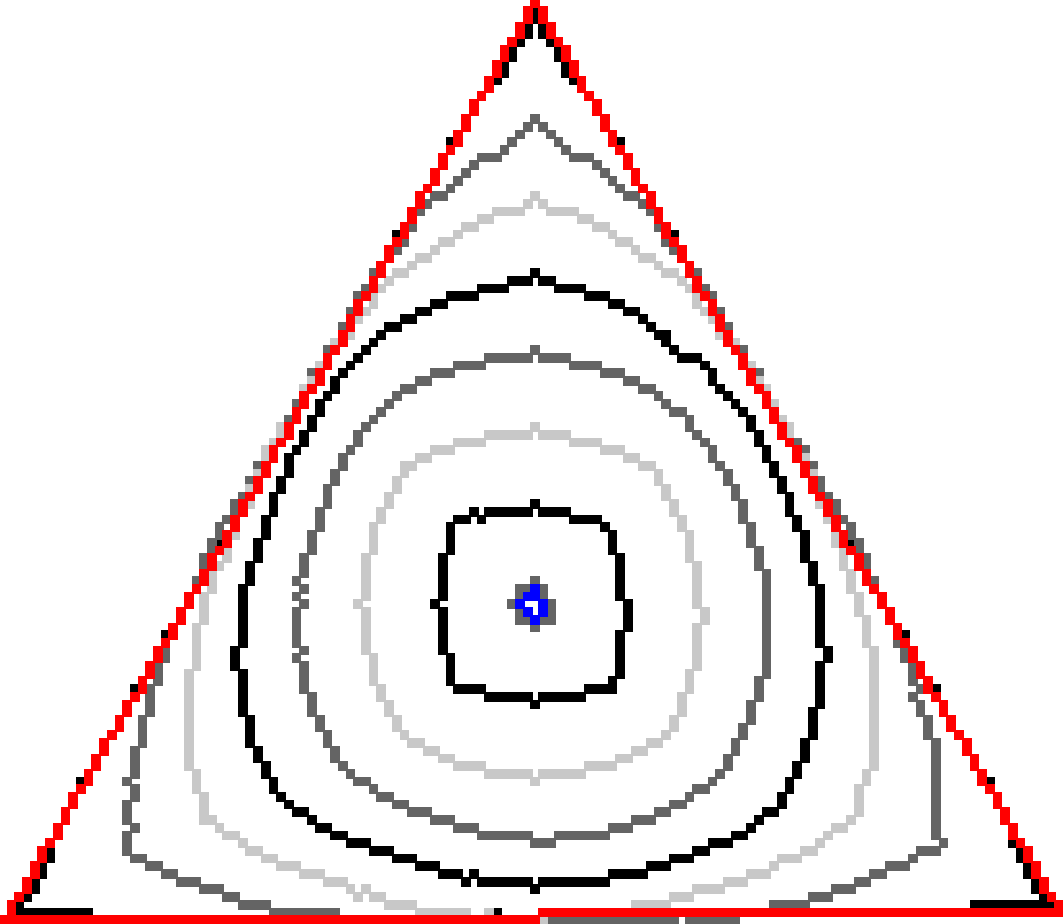
\includegraphics[scale=0.25]{figures/chapter7/balance-flow/triangle/summary.pdf} & 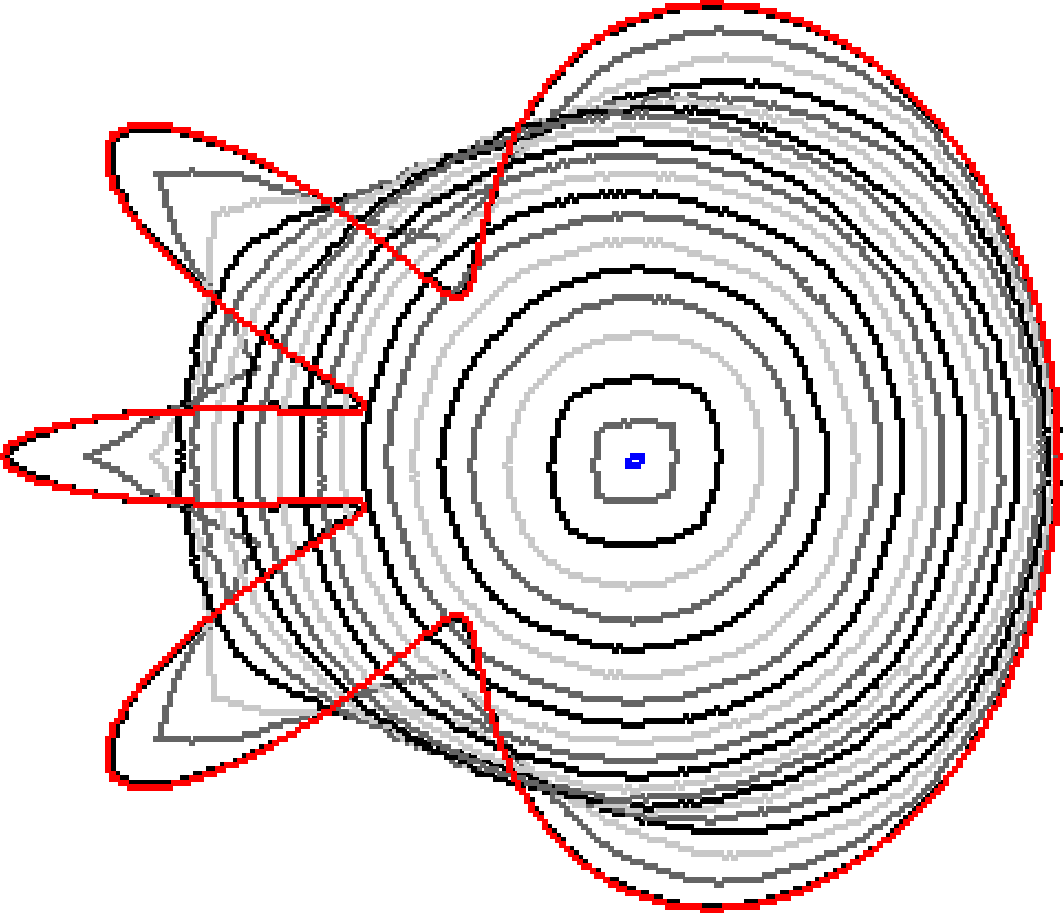
\includegraphics[scale=0.25]{figures/chapter7/balance-flow/flower/summary.pdf} & 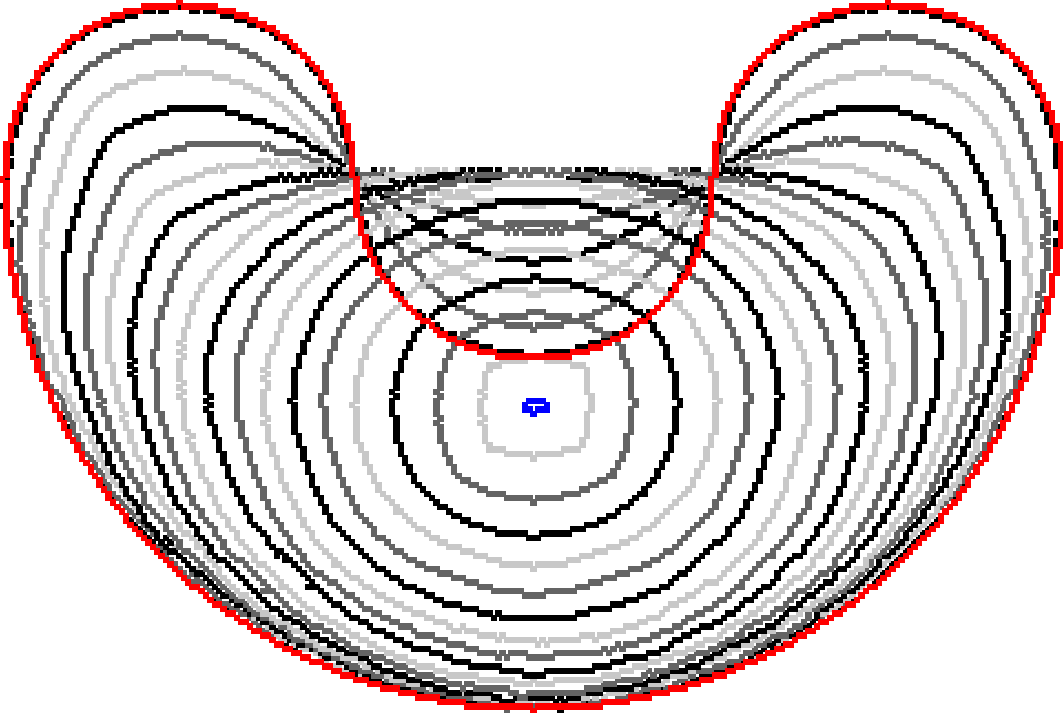
\includegraphics[scale=0.25]{figures/chapter7/balance-flow/bean/summary.pdf} \\
%$7$-FlipFlow & 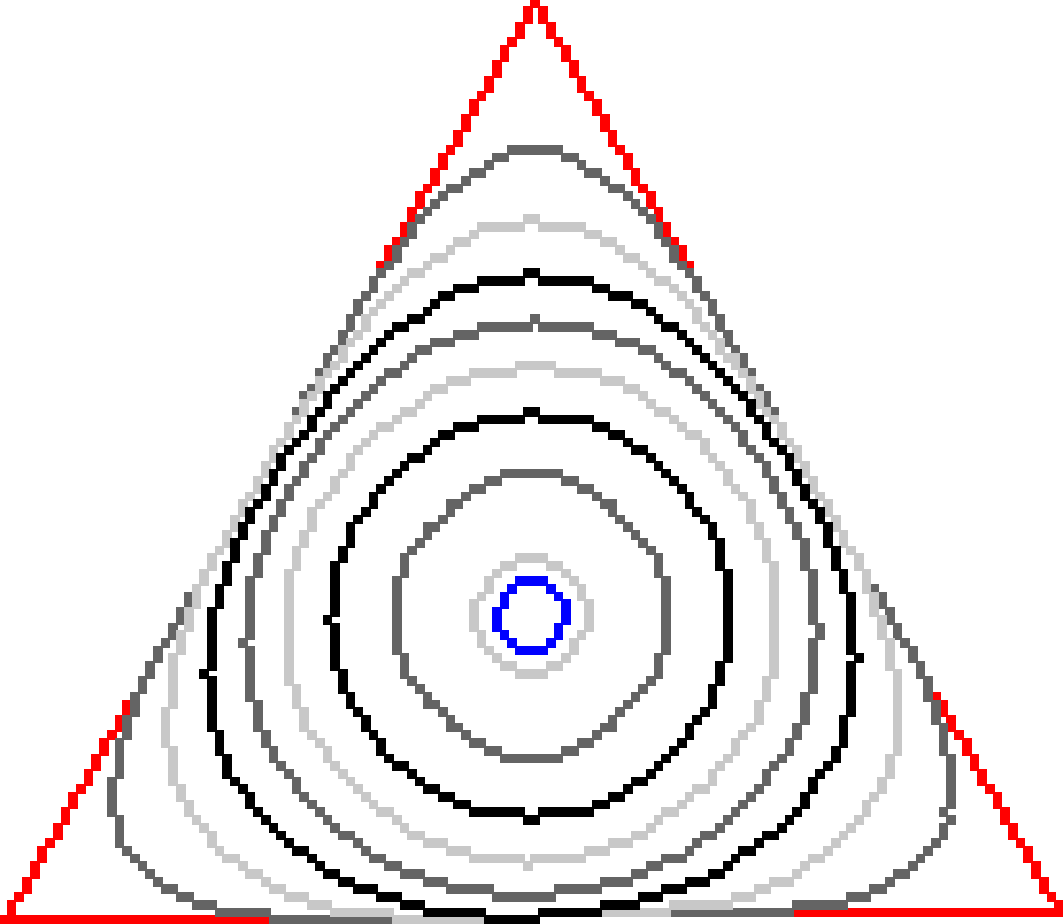
\includegraphics[scale=0.25]{figures/chapter7/flip-flow/triangle/summary.pdf} & 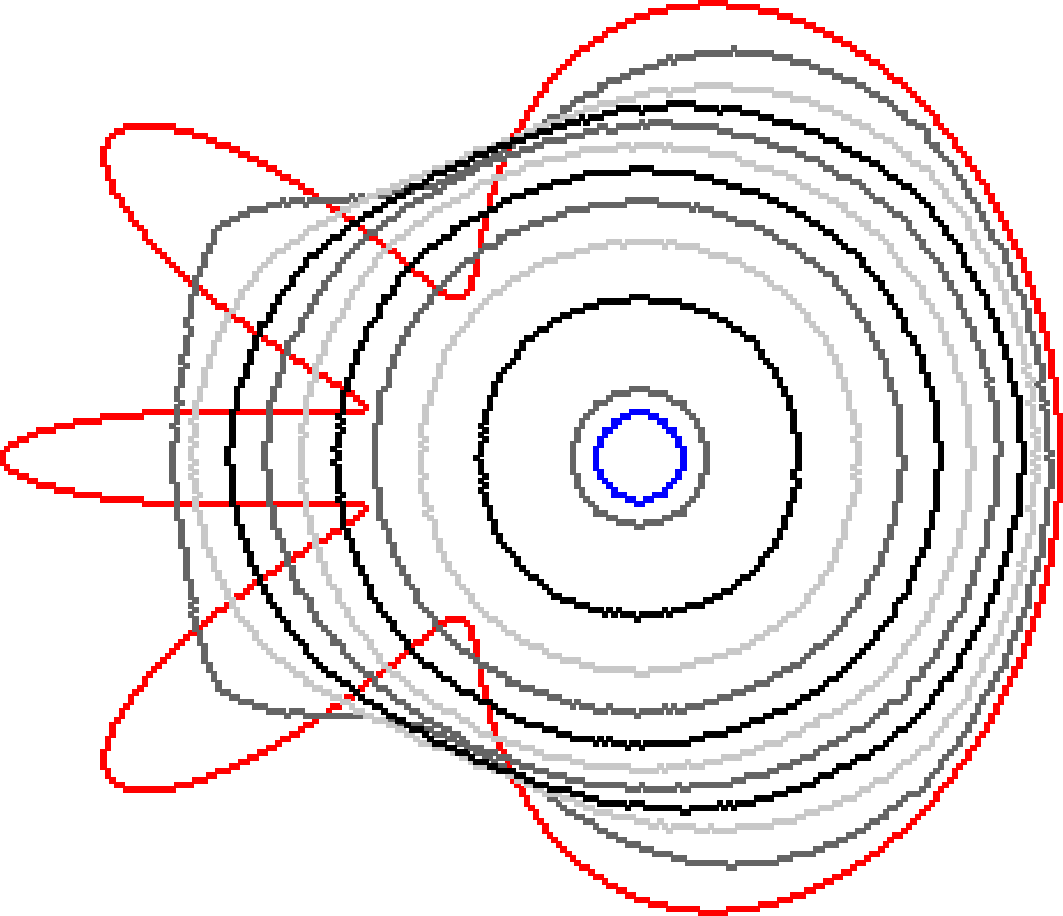
\includegraphics[scale=0.25]{figures/chapter7/flip-flow/flower/summary.pdf} & 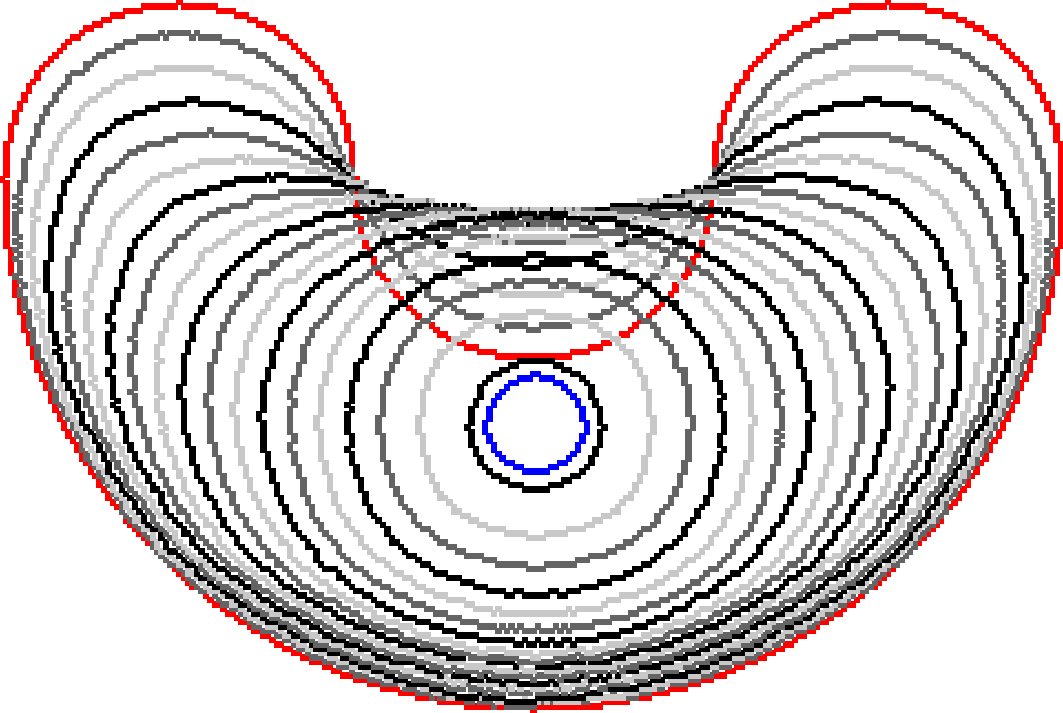
\includegraphics[scale=0.25]{figures/chapter7/flip-flow/bean/summary.pdf} \\
%\end{tabular}
%\caption{Evolutions of three shapes for the $7$-BalanceFlow and $7$-FlipFlow using a estimation ball radius of $9$. The models present similiar behaviour. Shapes are displayed at every $10$ iterations.}
%\label{fig:balance-flow-flip-flow-comparison}
%\end{figure}

\section{Towards a graph-based formulation}

%Let $A_o = \pi R^2 / 2 - |F_o|$ and $A_i = \pi R^2/2 - |F_i|$. We rewrite~\cref{eq:balance-term} as
%
%\begin{align*}
%	T_{m}^{bal}(\Ds) &= \Big(A_o - |X_o| + \sum_{x_j \in X_o}{x_j} \Big)^2 - \Big(A_i - \sum_{x_j \in X_i}{x_j}\Big)^2 \\
%	&= (A_o - |X_o|)^2 + 2(A_o - |X_o|)\sum_{x_j \in X_o}{x_j} +   \big(\sum_{x_j \in X_o}{x_j}\big)^2 - A_i^2  + 2A_i\sum_{x_j \in X_i}{x_j}  - \big(\sum_{x_j \in X_i}{x_j}\big)^2.
%\end{align*} 
%
%Grouping the constants in $c=(A_o - |X_o|)^2 - A_i^2$ and putting $x_j$ in evidence we obtain
%
%\begin{align}
%	T_{m}^{bal}(\Ds) 	&= c +\sum_{x_j \in X}{ 2x_j\Big( A_o - |X_o| + \frac{1}{2}\sum_{x_l \in X_o}{x_l} + A_i - \frac{1}{2}\sum_{x_l \in X_i}{x_l}\Big)} \nonumber \\
%	&= c +\sum_{x_j \in X}{2x_j\Bigg( \Big(A_o - \sum_{x_l \in X_o}{1-\frac{x_l}{2}}\Big) + \Big(A_i - \sum_{x_l \in X_i}{\frac{x_l}{2}}\Big)\Bigg)}.
%	\label{eq:xj-evidence}
%\end{align}
%
%We remark the similarity of the expression between parentheses in~\cref{eq:xj-evidence} and the sum $u(\Ds,p_o)^{1/2} + u(\Ds,p_i)^{1/2}$, i.e., the sum of balance coefficients square roots. The variable $x_j$ is set to zero if for every assignment for variables $x_l$, the expression in parentheses is greater than zero. That remark motivates us to define a graph-based model, described in the next chapter, in which the edge's weight are given by the sum of balance coefficients.

Looking at~\cref{fig:balance-plot} it would be interesting to find the point in which the inner or outer ball reaches the zero balance. In~\cref{fig:flower-balance-coefficient-zero-set} each color represents the balance coefficient $u_{12}$ of the closed shape with contour colored in white. We highlighted in magenta the pixels $p$ for which $u_{12}(\Ds,p) \leq 169$. ~\cref{fig:flower-balance-coefficient-zero-set} suggests that an evolution based on the zero level set of the balance coefficient may decrease the digital Elastica energy. In the next chapter we describe a graph-cut model in which the cost function is given by a function of the balance coefficients.

\begin{figure}
\center
\includegraphics[scale=0.05]{figures/chapter7/level-set/flower.pdf}
\caption{Balance coefficient map of radius $12$ for the flower shape (contour in white). The pixels in magenta have balance coefficient smaller than $169$. }
\label{fig:flower-balance-coefficient-zero-set}
\end{figure}


\section{Conclusion}
The BalanceFlow model is closely related to the FlipFlow but it has a simple implementation and interpretation. The balance coefficent is the link that connects both models and the motivation for the graph-cut model proposed in the next chapter.




